\section{Ähnlichkeit im Raum}\index{Ähnlichkeit!im Raum}
\sectuntertitel{``Na Anna, was hat dir dein Bruder zum Geburtstag
  geschenkt?'' - ``Ein leeres Sparschwein!'' - ``Das sieht ihm mal wieder
  ähnlich!'' - ``Nein, eigentlich kein bißchen!''}

\theorieTALSGeom{171}{3.4}

\subsection*{Lernziele}
\begin{itemize}
\item Streckungsfaktor (analog 2d)
\end{itemize}
\newpage

\subsection{Streckungsfaktor}

\begin{tabular}{cc}
  $K$ & $K'$ \\
  \hline
  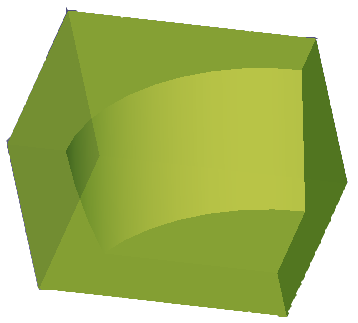
\includegraphics[width=4cm]{tals/stereo/img/aehnlich_klein.png} & 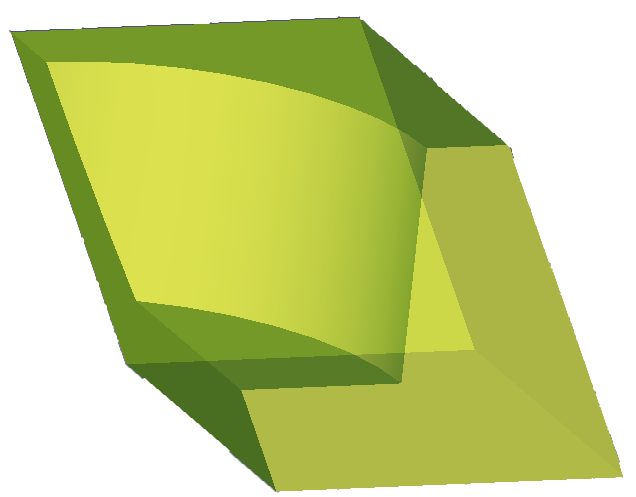
\includegraphics[width=6cm]{tals/stereo/img/aehnlich_gross.png}\\

  \end{tabular} 

Sei $K$ der Originalkörper und $K'$ der gestreckte, ähnliche Körper, dann gilt
für die Volumen ($V$ und $V'$), die Flächen ($A$ und $A'$) und
die Strecken ($a$ und $a'$) folgendes Gesetz:

\begin{gesetz}{}{}
  Der (lineare) Streckungsfaktor sei $k$.

  $$a \cdot{} k^1 = a'$$

  $$A \cdot{} k^2 = A'$$
  $$V \cdot{} k^3 = V'$$
\end{gesetz}

\begin{bemerkung}{Volumina}{}
Der Exponent beim Streckungsfaktor $k$ entspricht der \textbf{Dimension!Ähnlichkeit}\index{Dimension} der
betrachteten «Volumina». Dabei ist das \textbf{zweidimensionale Volumen}\index{Volumen!Ähnlichkeit} die
Fläche während die Streckenlänge das \textbf{eindimensionale Volumen} darstellt.
\end{bemerkung}

\begin{bemerkung}{Verhältnisse}{}
  $$k = \frac{a'}{a} = \sqrt{\frac{A'}{A}} = \sqrt[3\,\,\,]{\frac{V'}{V}}$$
\end{bemerkung}

  
\newpage
